\documentclass{beamer}
\usepackage[utf8]{inputenc}
\usepackage[T1]{fontenc}
\usepackage{amsmath}
\usepackage{graphicx}
\usepackage{lmodern}
\usepackage{listings}
\usepackage{xcolor}
\usepackage{hyperref}
\usepackage{tikz}
\usepackage[style=verbose, backend=bibtex]{biblatex} % style=verbose affiche tout en bas de slide
\addbibresource{references.bib} % Indique ton fichier de bibliographie

\graphicspath{{img/}}
\setbeamertemplate{footline}[frame number]
\lstset{
    basicstyle=\ttfamily\footnotesize,
    keywordstyle=\color{blue},
    stringstyle=\color{red},
    showstringspaces=false
}
\hypersetup{
    colorlinks=true,
    linkcolor=blue,
    filecolor=magenta,
    urlcolor=cyan,
    pdftitle={Présentation — Méthode SIFT},
    pdfpagemode=FullScreen,
}

\title{Projet RL}
\subtitle{Colorisation d'image N/B}
\author{Louis LENOBLE, Dylan SANSON, Yohann DELAPLACE}
\date{\today}

% Mini-sommaire automatique à chaque début de section
\AtBeginSection[]{
  \begin{frame}{Sommaire}
    \tableofcontents[currentsection, hideothersubsections]
  \end{frame}
}

\setcounter{tocdepth}{2}

\begin{document}

\begin{frame}
    \titlepage
\end{frame}

\setcounter{tocdepth}{1} % 1 = section, 2 = subsection, 3 = subsubsection

% Sommaire global
\begin{frame}{Sommaire}
    \tableofcontents
\end{frame}

%------------------------------------------------------------------------------------------------------------------------------------------------------------

\section{Spécifications}
\subsection{Objectif}

%------------------------------------------------------------------------------------------------------------------------------------------------------------

\begin{frame}{Objectif}
    \begin{columns}[c] % [c] pour l'alignement vertical centré
        
        % Colonne de gauche : Image Noir et Blanc
        \begin{column}{0.42\textwidth}
            \begin{figure}
                \centering
                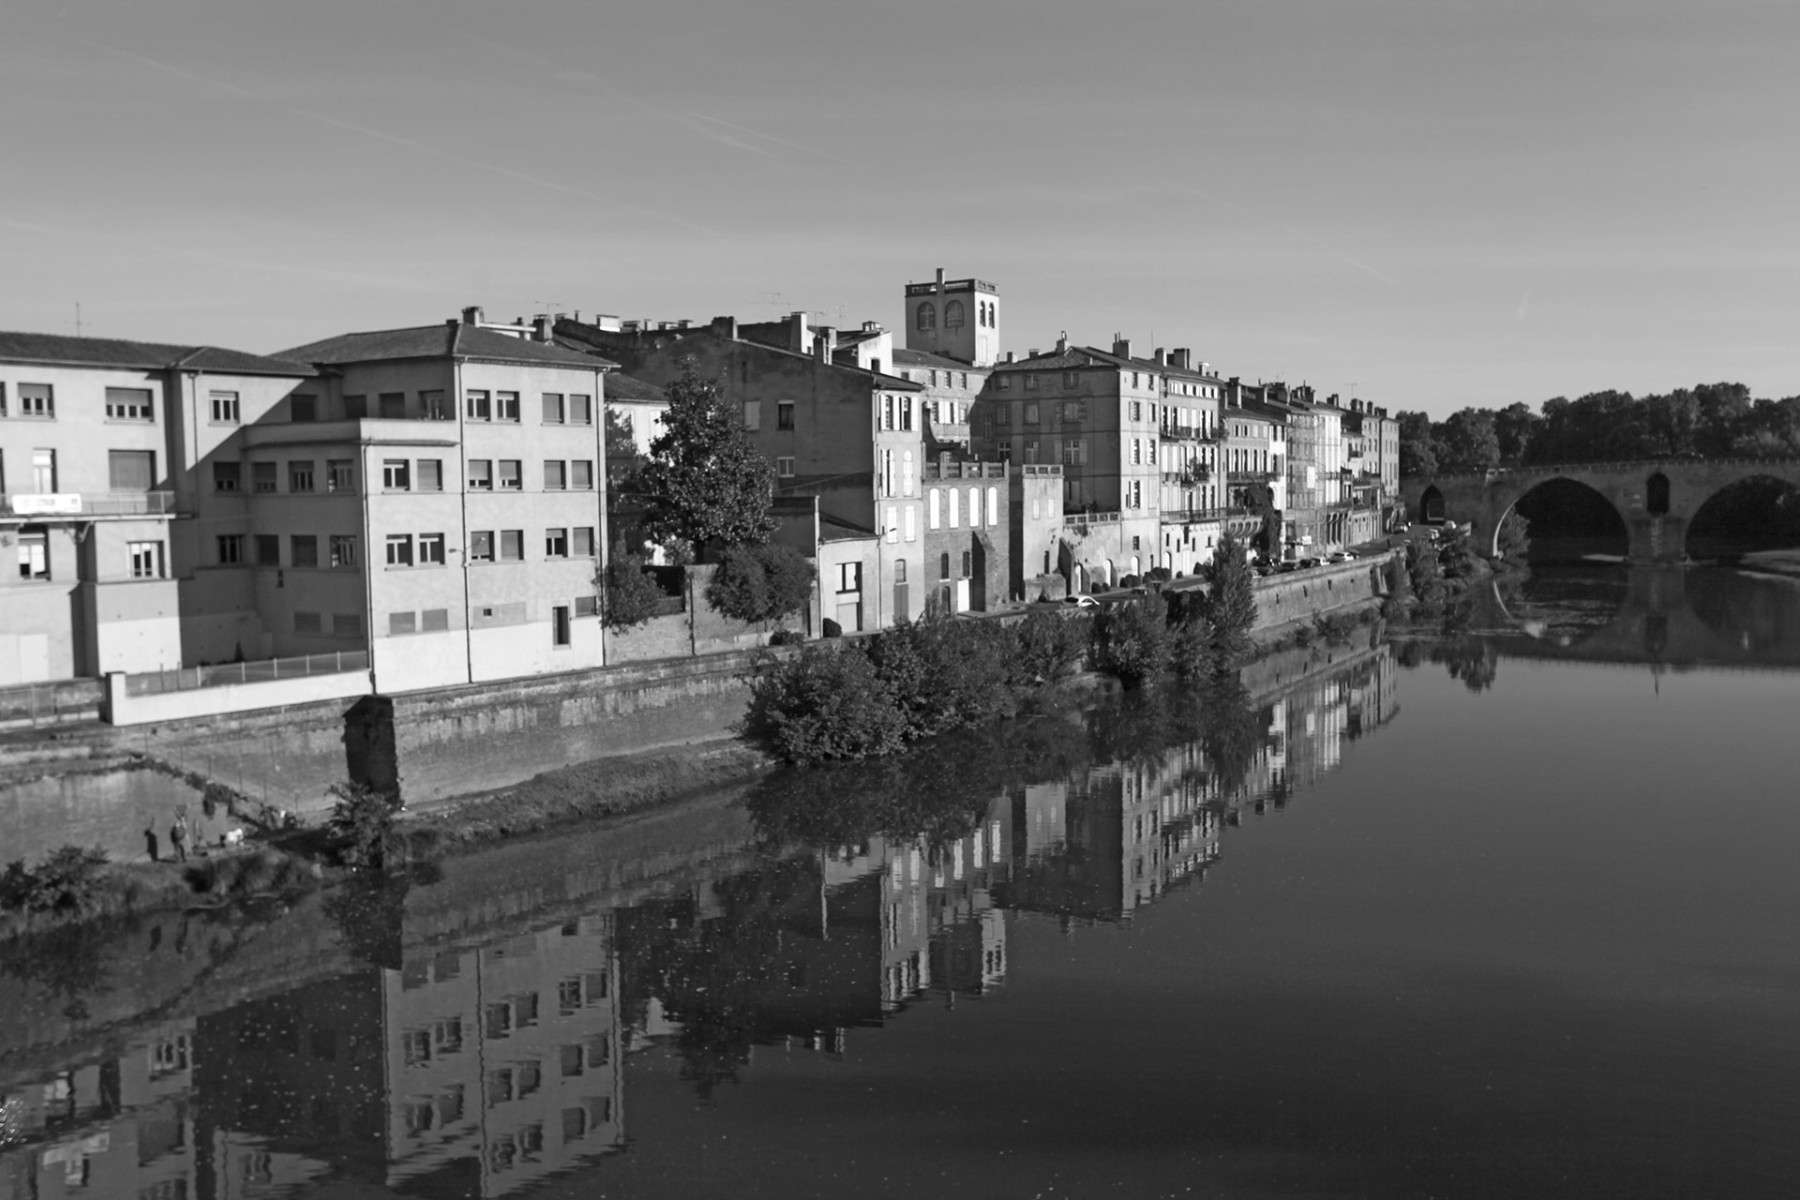
\includegraphics[width=\textwidth]{img/image_exemple_NB.jpg}
                \caption{Image d'entrée (N\&B)}
            \end{figure}
        \end{column}

        % Colonne centrale : La flèche de transition
        \begin{column}{0.1\textwidth}
            \centering
            \tikz \draw[-stealth, red, line width=2pt, bend left=20] (0,0) to (1,0);
        \end{column}

        % Colonne de droite : Image Colorisée
        \begin{column}{0.42\textwidth}
            \begin{figure}
                \centering
                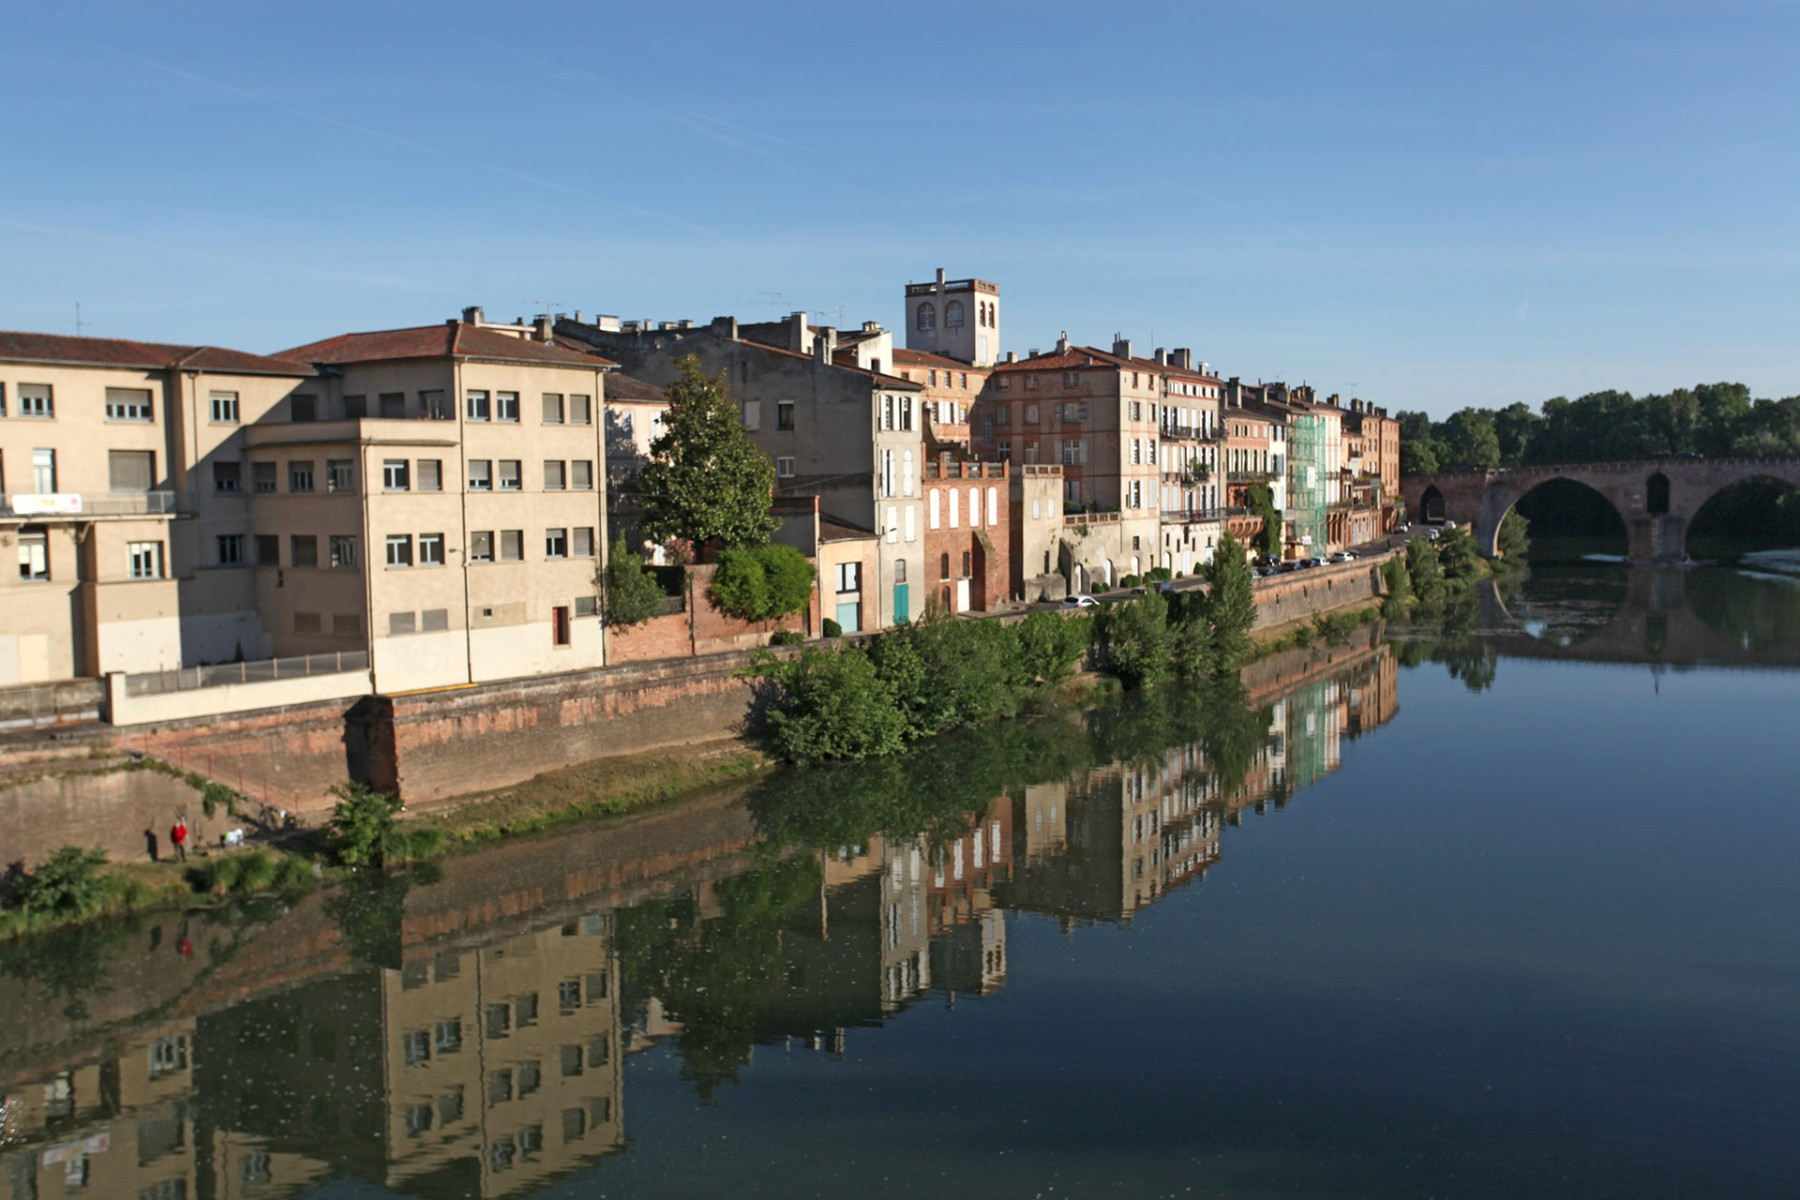
\includegraphics[width=\textwidth]{img/image_exemple_couleur.jpg}
                \caption{Image traitée (Couleur)}
            \end{figure}
        \end{column}

    \end{columns}
\end{frame}


%------------------------------------------------------------------------------------------------------------------------------------------------------------

\subsection{Formalisation du problème}

%------------------------------------------------------------------------------------------------------------------------------------------------------------

\begin{frame}{Choix de l'espace colorimétrique}
    L'utilisation de l'espace Lab est privilégiée par rapport au RGB.

    \vfill 

    \begin{itemize}
        \item \textbf{L} (Luminance) : Représente l'intensité lumineuse (l'image en noir et blanc). C'est notre \textbf{donnée d'entrée}.
        \item Canaux \textbf{a} et \textbf{b} (Chrominance) : Représentent les composantes de couleur (axe vert-rouge et axe bleu-jaune). Ce sont nos \textbf{inconnues}. 
    \end{itemize}
\end{frame}


%------------------------------------------------------------------------------------------------------------------------------------------------------------

\begin{frame}{Métriques d'évaluation : MAE}

\begin{itemize}
    \item \textbf{Calcul de base }: Le MAE est obtenu en calculant la moyenne de l'erreur absolue entre l'image générée par le modèle et l'image source originale.

    \item \textbf{Niveau de précision} : Ce calcul s'effectue au niveau de chaque pixel pour chaque canal de couleur.

    \item \textbf{Interprétation} : Plus la valeur du MAE est basse, plus l'image colorisée est proche de la vérité terrain (l'image originale).


\end{itemize}

\begin{equation}
    MAE = \frac{1}{3n} \sum_{l=1}^{3} \sum_{p=1}^{n} |h(x)^{(p,l)} - y^{(p,l)}|
\end{equation}

% Définition des termes :
% n : nombre total de pixels
% l : indice des canaux de couleur (L, a, b) 
% h(x) : valeur prédite par le modèle pour le pixel p et le canal l
% y : valeur réelle (ground truth) pour le pixel p et le canal l
    
\end{frame}

%------------------------------------------------------------------------------------------------------------------------------------------------------------

\begin{frame}{Métriques d'évaluation : Accuracy}

\begin{itemize}
    \item \textbf{Calcul de base} : L'accuracy est définie comme le ratio entre le nombre de pixels possédant la même information de couleur que l'image source et le nombre total de pixels $n$.
    
    \item \textbf{Critère de précision} : Un pixel est considéré comme correct si la différence absolue entre ses canaux de couleur prédits et ceux de l'image originale est inférieure à un seuil de distance déterminé $\epsilon$.
    
    \item \textbf{Interprétation} : Plus la valeur de l'accuracy est élevée, plus le modèle est performant dans sa capacité à reconstruire fidèlement les couleurs originales de la vérité terrain.
\end{itemize}

\begin{equation}
    acc(x,y) = \frac{1}{n} \sum_{p=1}^{n} \prod_{l=1}^{s} {\textbf{1}}_{[0,\epsilon_{l}]} (|h(x)^{(p,l)} - y^{(p,l)}|)
\end{equation}
    
\end{frame}

%------------------------------------------------------------------------------------------------------------------------------------------------------------

\section{Conception du modèle}

\subsection{Qu'est-ce qu'un GAN ?}

%------------------------------------------------------------------------------------------------------------------------------------------------------------

\begin{frame}{Utilisation d'un GAN}

    Proposé en 2014 par \textbf{Goodfellow et al.} \footcite{goodfellow2014} :

    \begin{figure}
        \centering
        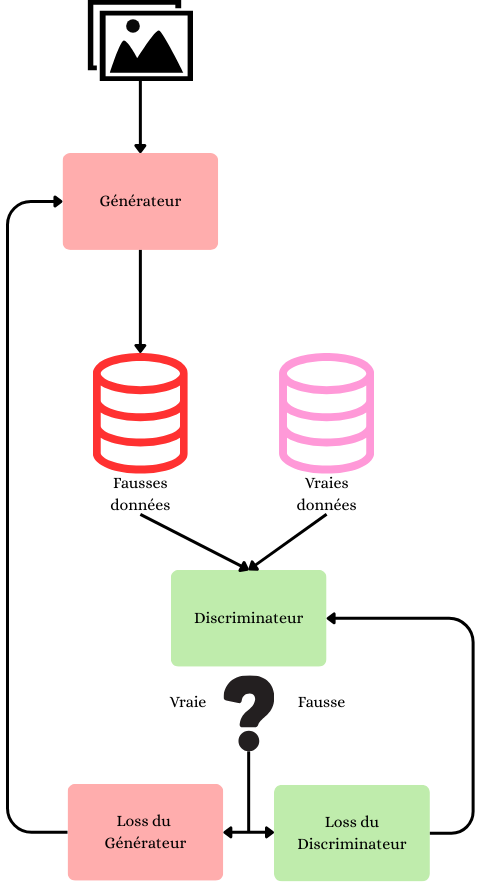
\includegraphics[width=0.33\textwidth]{img/schema_GAN.png}
        \caption{Schéma de la structure d'un GAN}
    \end{figure}

    
\end{frame}

%------------------------------------------------------------------------------------------------------------------------------------------------------------

\subsection{Le GAN pour les images}

\begin{frame}{Le générateur et discriminateur}

    \textbf{Isola et al.} \footcite{isola2017pix2pix} propose en 2018 une architecture généralisée pour de nombreux problèmes d'imagerie :

    \begin{figure}
        \centering
        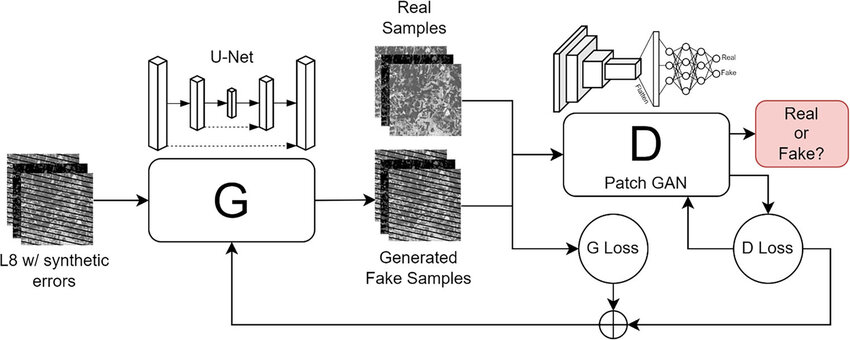
\includegraphics[width=0.70\textwidth]{img/Pix2Pix.png}
        \caption{Architecture GAN proposée par Pix2Pix}
    \end{figure}

\end{frame}

%------------------------------------------------------------------------------------------------------------------------------------------------------------

\subsection{Implémentation pour la colorisation d'images}

\begin{frame}{Exemple d'implémentation d'une architecture similaire pour la colorisation d'image}

    Plus tard en 2018, \textbf{Nazeri et al.} \footcite{nazeri2018image}  propose une implémentation de cette architecture, spécifiquement pour la colorisation d'image :

    \begin{figure}
        \centering
        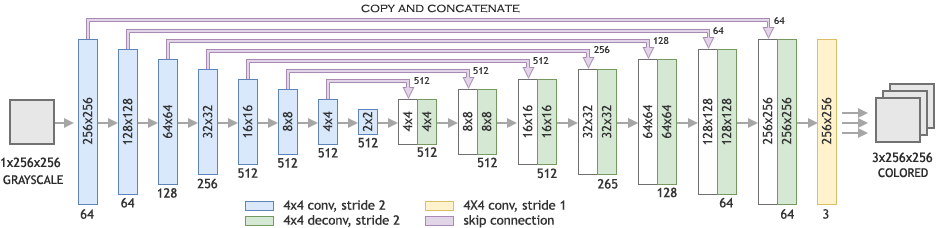
\includegraphics[width=1.0\textwidth]{img/unet_implementation.png}
        \caption{Générateur U-net utilisé}
    \end{figure}

\end{frame}

%------------------------------------------------------------------------------------------------------------------------------------------------------------
\section{Implémentation et résultats}
\subsection{Dataset}
%------------------------------------------------------------------------------------------------------------------------------------------------------------
\begin{frame}{Dataset utilisé}
    \begin{center}
    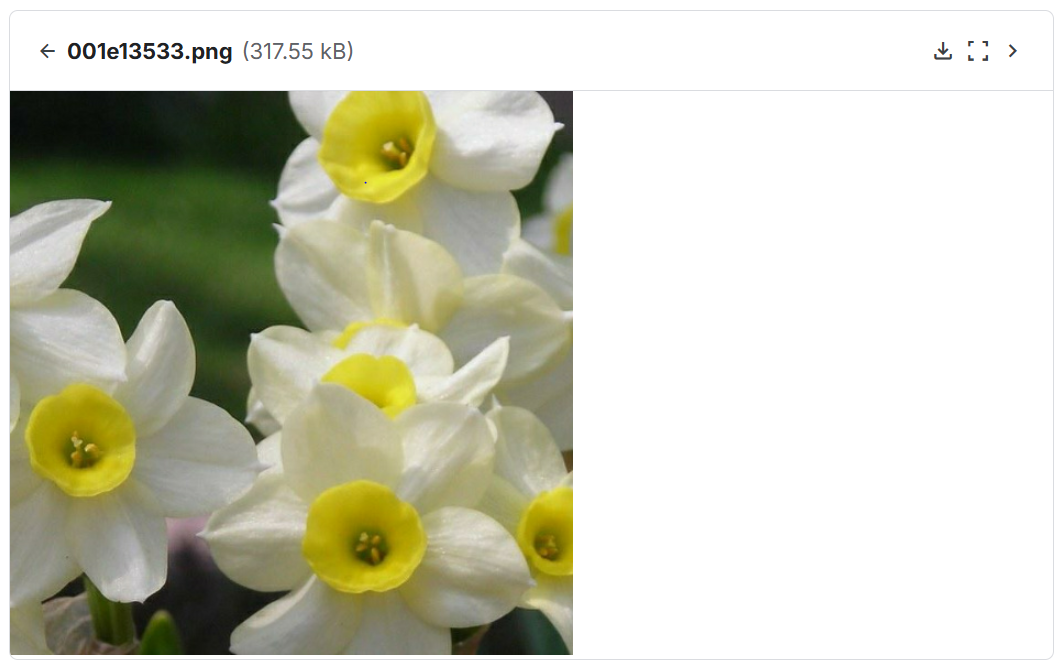
\includegraphics[width=0.8\linewidth]{dataset.PNG}
    \end{center}

    https://www.kaggle.com/datasets/alenic/flower-classification-512-png
\end{frame}

%------------------------------------------------------------------------------------------------------------------------------------------------------------
\begin{frame}{Pré-traitements}
    \begin{itemize}
        \item Passage RGB en Lab
        \item Réduction de la résolution de 512 à 256 pixels
        \item Normalisation : [0, 255] → [-1, 1]
    \end{itemize}
\end{frame}
%------------------------------------------------------------------------------------------------------------------------------------------------------------
\begin{frame}{Data augmentation}
    \begin{center}
        \begin{figure}
            \centering
            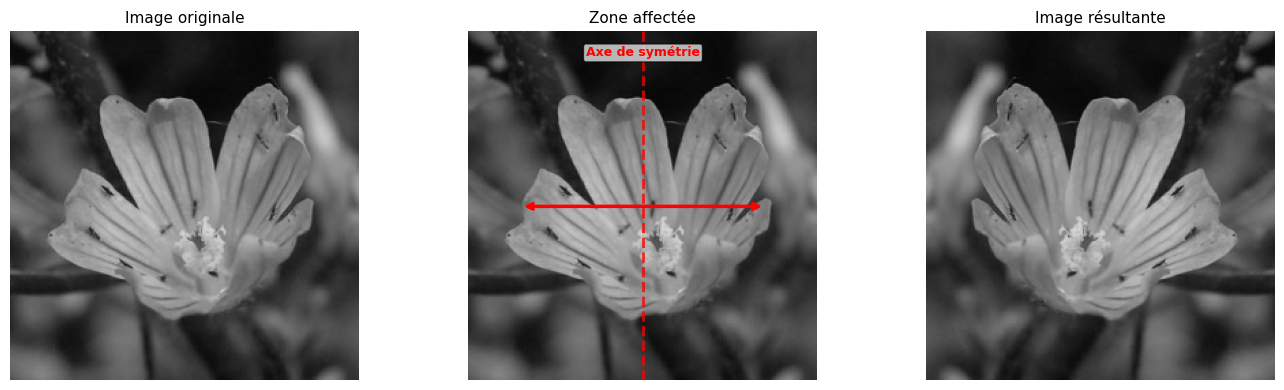
\includegraphics[height=0.3\textheight]{img/flip.png}
            \caption{Opération de flip horizontal}
        \end{figure}

        \vfill
        
        \begin{figure}
            \centering
            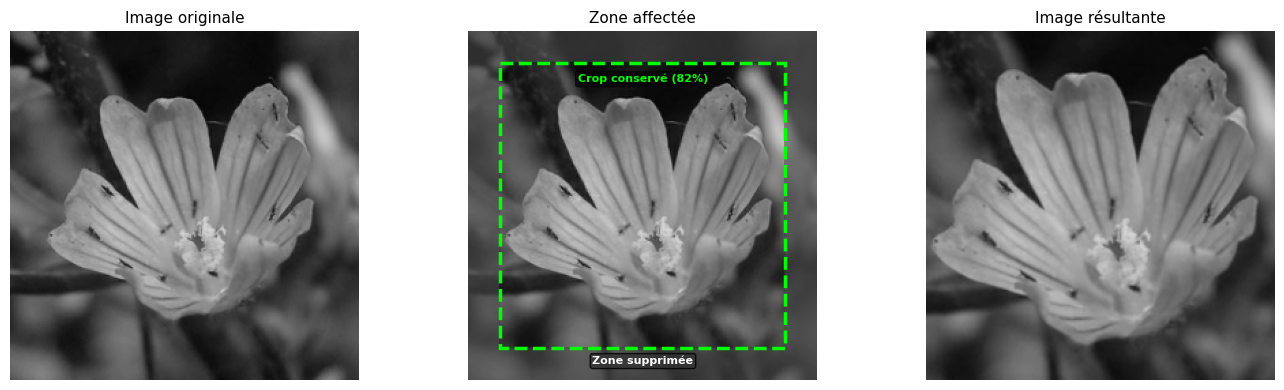
\includegraphics[height=0.3\textheight]{img/crop.png}
            \caption{Opération de crop}
        \end{figure}
    \end{center}
\end{frame}
%------------------------------------------------------------------------------------------------------------------------------------------------------------
\begin{frame}{Data augmentation}
    \begin{center}
        \begin{figure}
            \centering
            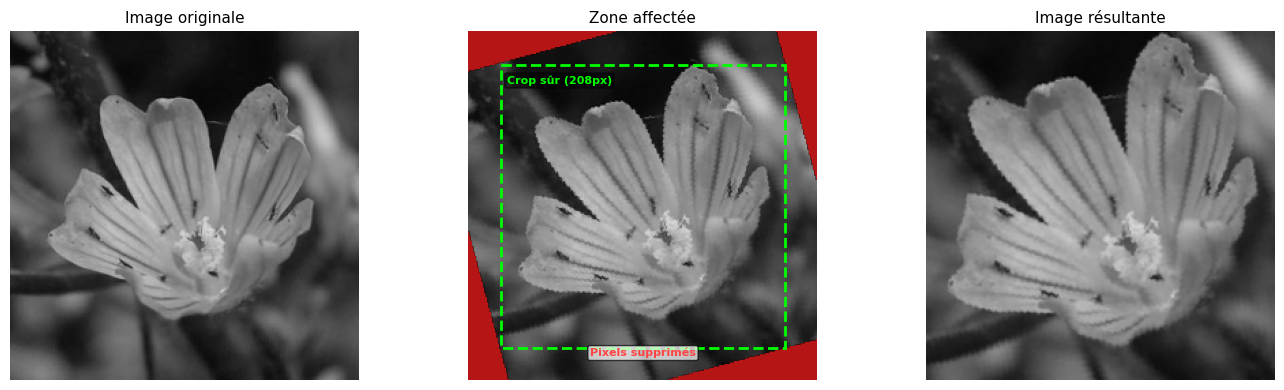
\includegraphics[height=0.3\textheight]{img/rotation_crop.png}
            \caption{Opération de rotation et de crop}
        \end{figure}

        \vfill
        
        \begin{figure}
            \centering
            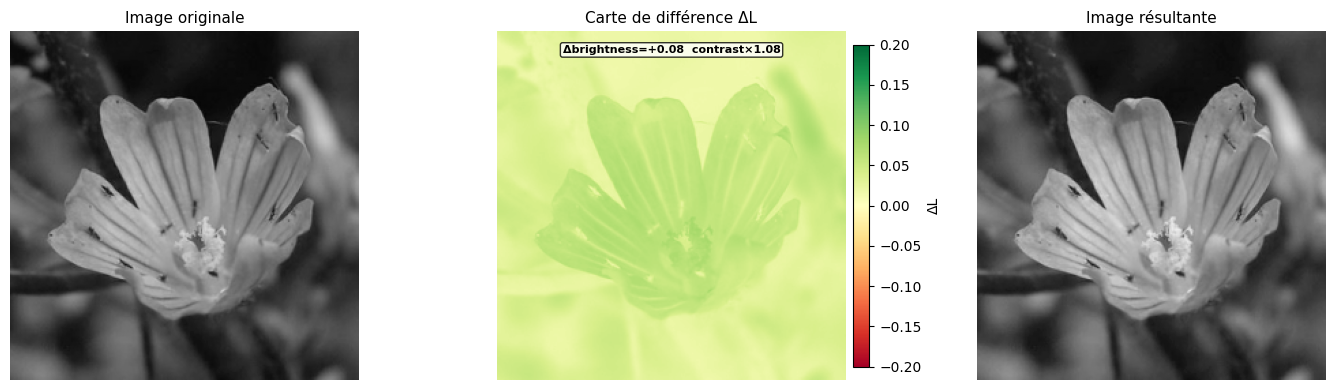
\includegraphics[height=0.3\textheight]{img/jitter.png}
            \caption{Opération de jitter de luminosité}
        \end{figure}
    \end{center}
\end{frame}
%------------------------------------------------------------------------------------------------------------------------------------------------------------
\subsection{Entraînement}
%------------------------------------------------------------------------------------------------------------------------------------------------------------
\begin{frame}{Hyper-paramètres}
\begin{itemize}
    \item \color{red} \textbf{Paramètre de régularisation ($\lambda$)} : $100$. 
    \item \color{red} \textbf{Taux d'apprentissage initial} : $2 \times 10^{-4}$. 
    
    \item \color{black}\textbf{Facteur de décroissance du taux d'apprentissage} : $10$. 
    \item \textbf{Pente Leaky-ReLU} : $0.2$. 
    \item \textbf{Filtres de convolution et stride} : Convolutions de $4 \times 4$ avec un pas de $2$. 
    \item \textbf{Label smoothing} : $0.9$ pour les étiquettes positives, $0$ pour les négatives. 
    \item \textbf{Terme de momentum Adam ($\beta_1$)} : $0.5$. 
    \item \color{red}\textbf{Batch Size} : $128$ pour CIFAR-10, $16$ pour Places365.
    \item \color{red}\textbf{Nombre d'epochs} : $200$ pour CIFAR-10, $20$ pour Places365.
\end{itemize}
\end{frame}
%------------------------------------------------------------------------------------------------------------------------------------------------------------
\begin{frame}{Quelques courbes de loss intéressantes}
    \begin{columns}[c] % [c] pour l'alignement vertical centré
        
        
        % Colonne de gauche : Première courbe
        \begin{column}{0.50\textwidth}
            \begin{figure}
                \centering
                \includegraphics[width=\textwidth]{img/train_epoch_ponderation.png}
                \caption{Courbe d'entrainement avec la pondération manuelle de la loss}
            \end{figure}
        \end{column}
        
        
        % Colonne de droite : deuxieme courbe
        \begin{column}{0.50\textwidth}
            \begin{figure}
                \centering
                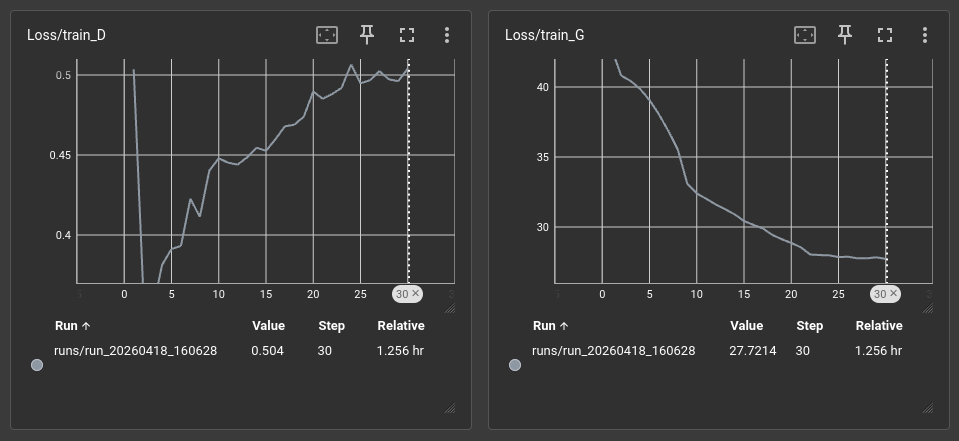
\includegraphics[width=\textwidth]{img/perception_epoch.png}
                \caption{Courbe d'entrainement avec la perceptual loss et la pondération}
            \end{figure}
        \end{column}

        

    \end{columns}
\end{frame}
%------------------------------------------------------------------------------------------------------------------------------------------------------------
\subsection{Résultats}

%------------------------------------------------------------------------------------------------------------------------------------------------------------
\begin{frame}{Résultats : Image d'exemple en couleur}
    \begin{figure}
        \centering
        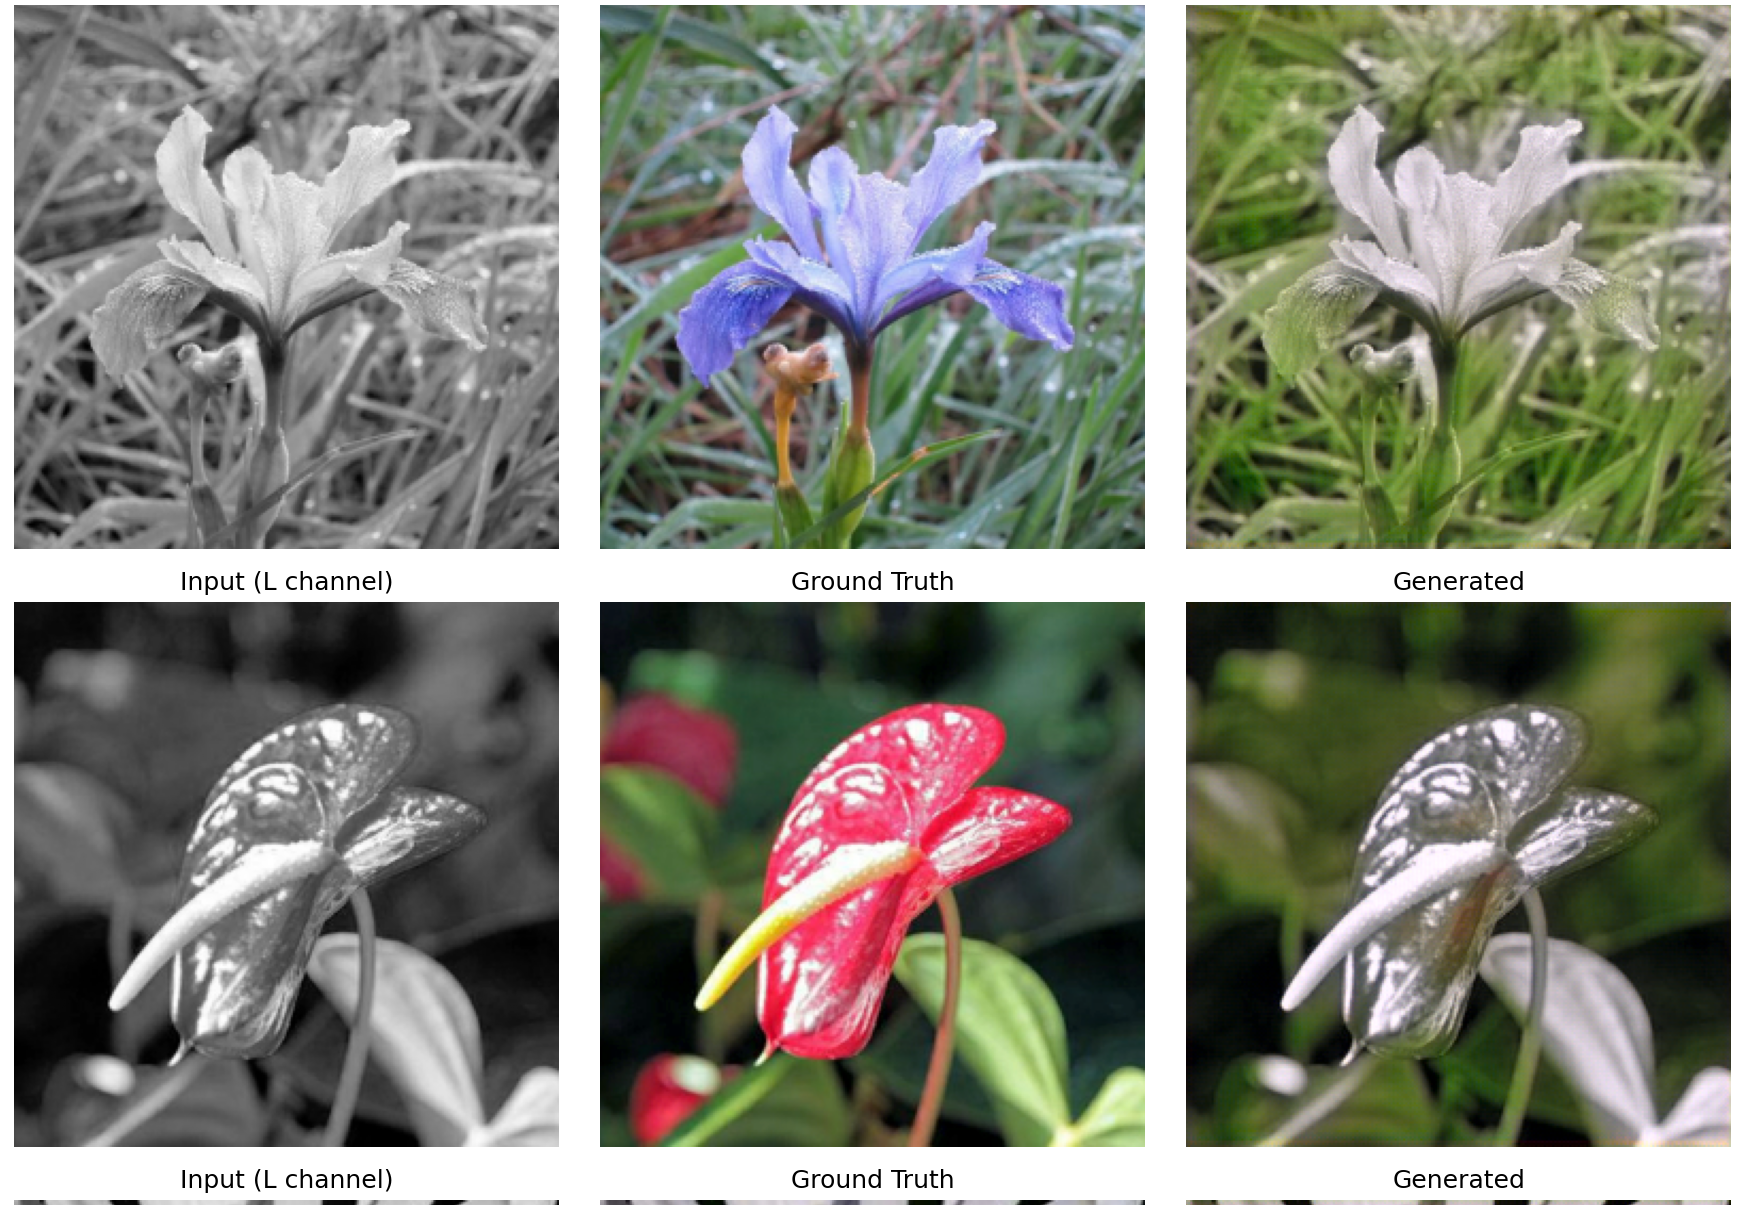
\includegraphics[width=0.9\textwidth, height=0.7\textheight, keepaspectratio]{img/exemple_epoch1.png}
        \caption{Image source en couleur}
    \end{figure}
\end{frame}

\begin{frame}{Résultats : Ajustement du Learning Rate}
    \begin{figure}
        \centering
        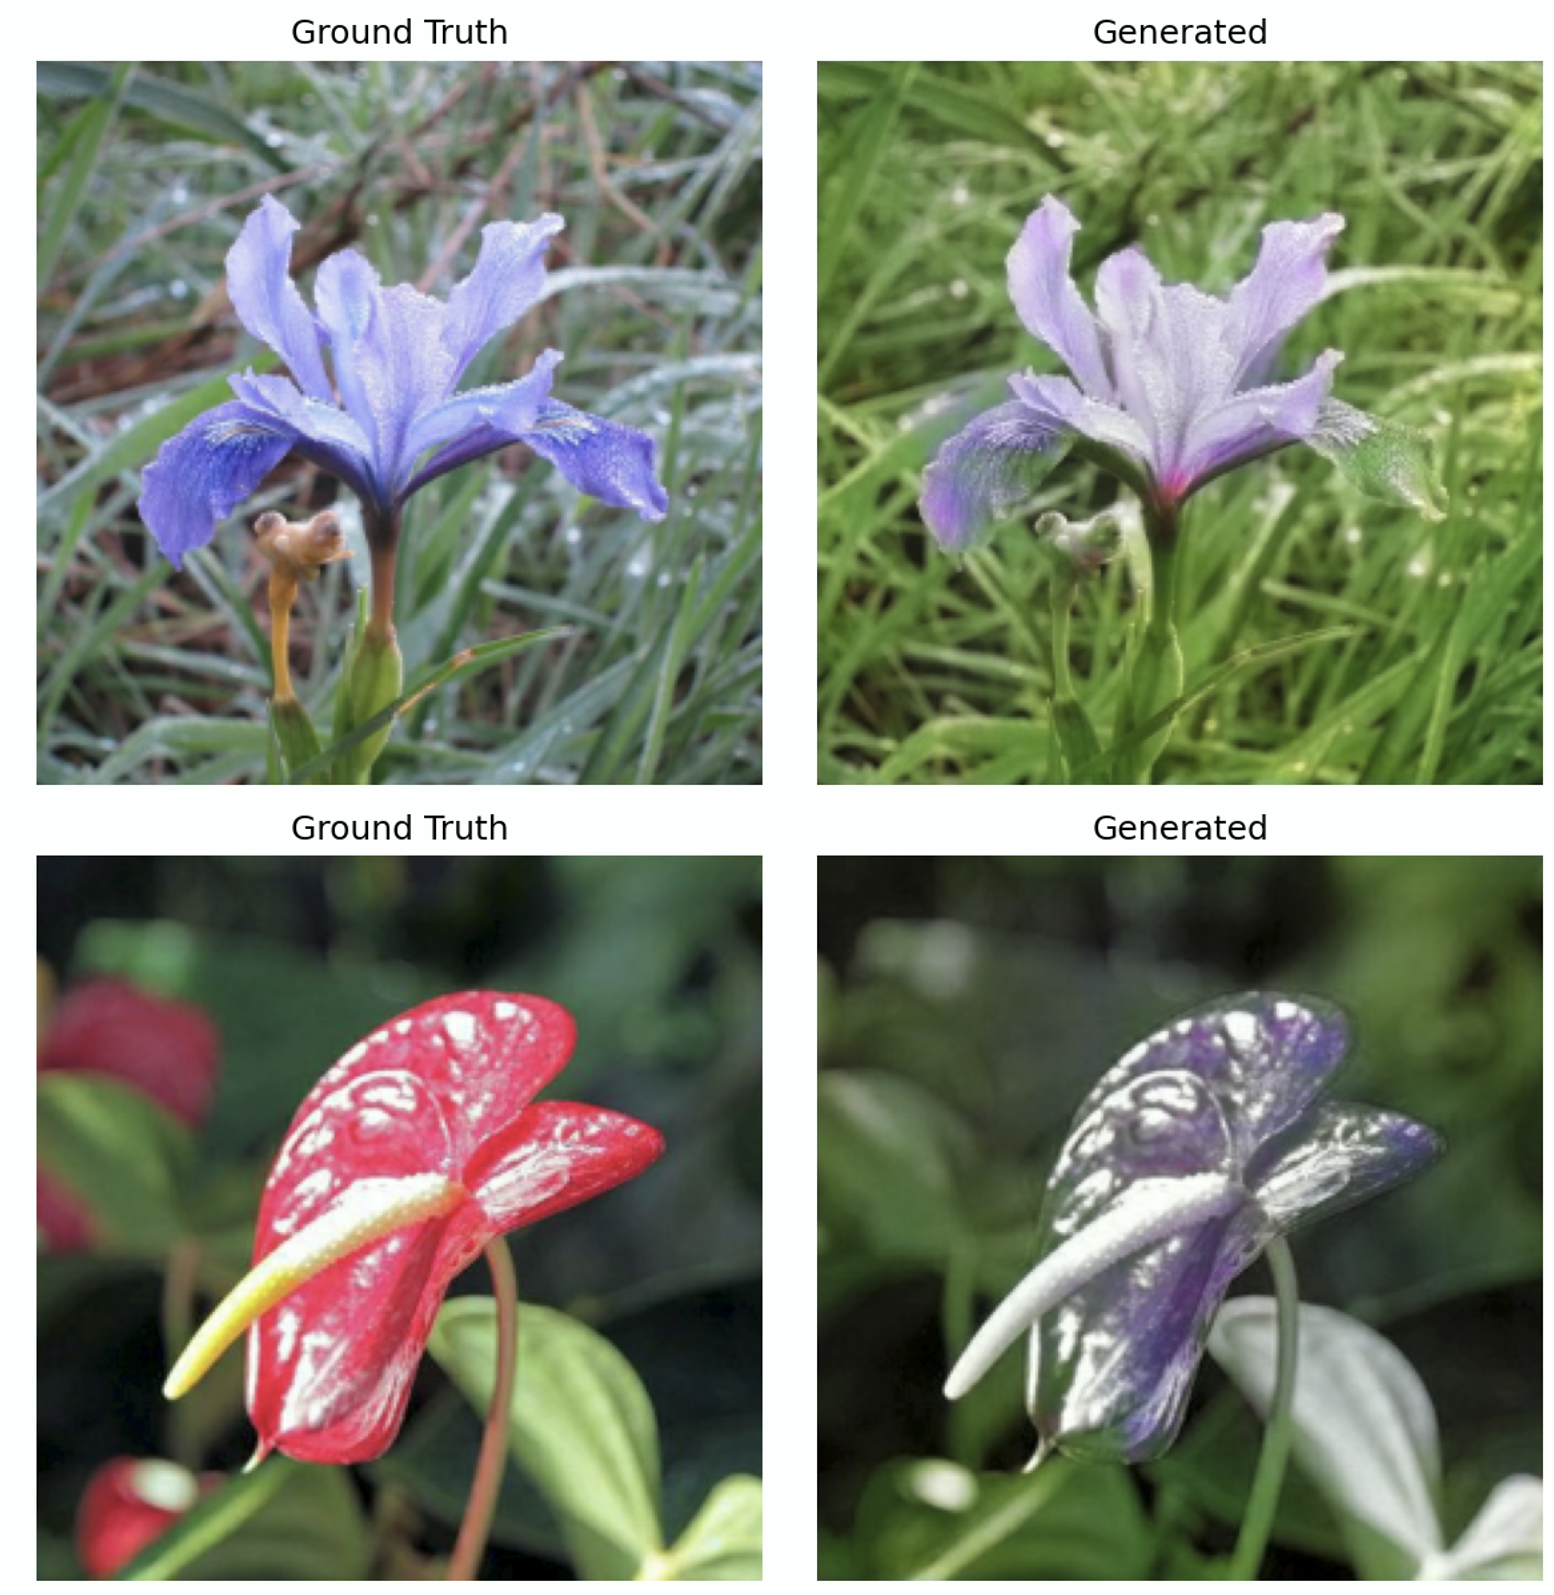
\includegraphics[width=0.9\textwidth, height=0.7\textheight, keepaspectratio]{img/lr_validation_epoch020.png}
        \caption{Validation avec optimisation du learning rate}
    \end{figure}
\end{frame}

\begin{frame}{Résultats : Impact des paramètres Lambda et Learning Rate}
    \begin{figure}
        \centering
        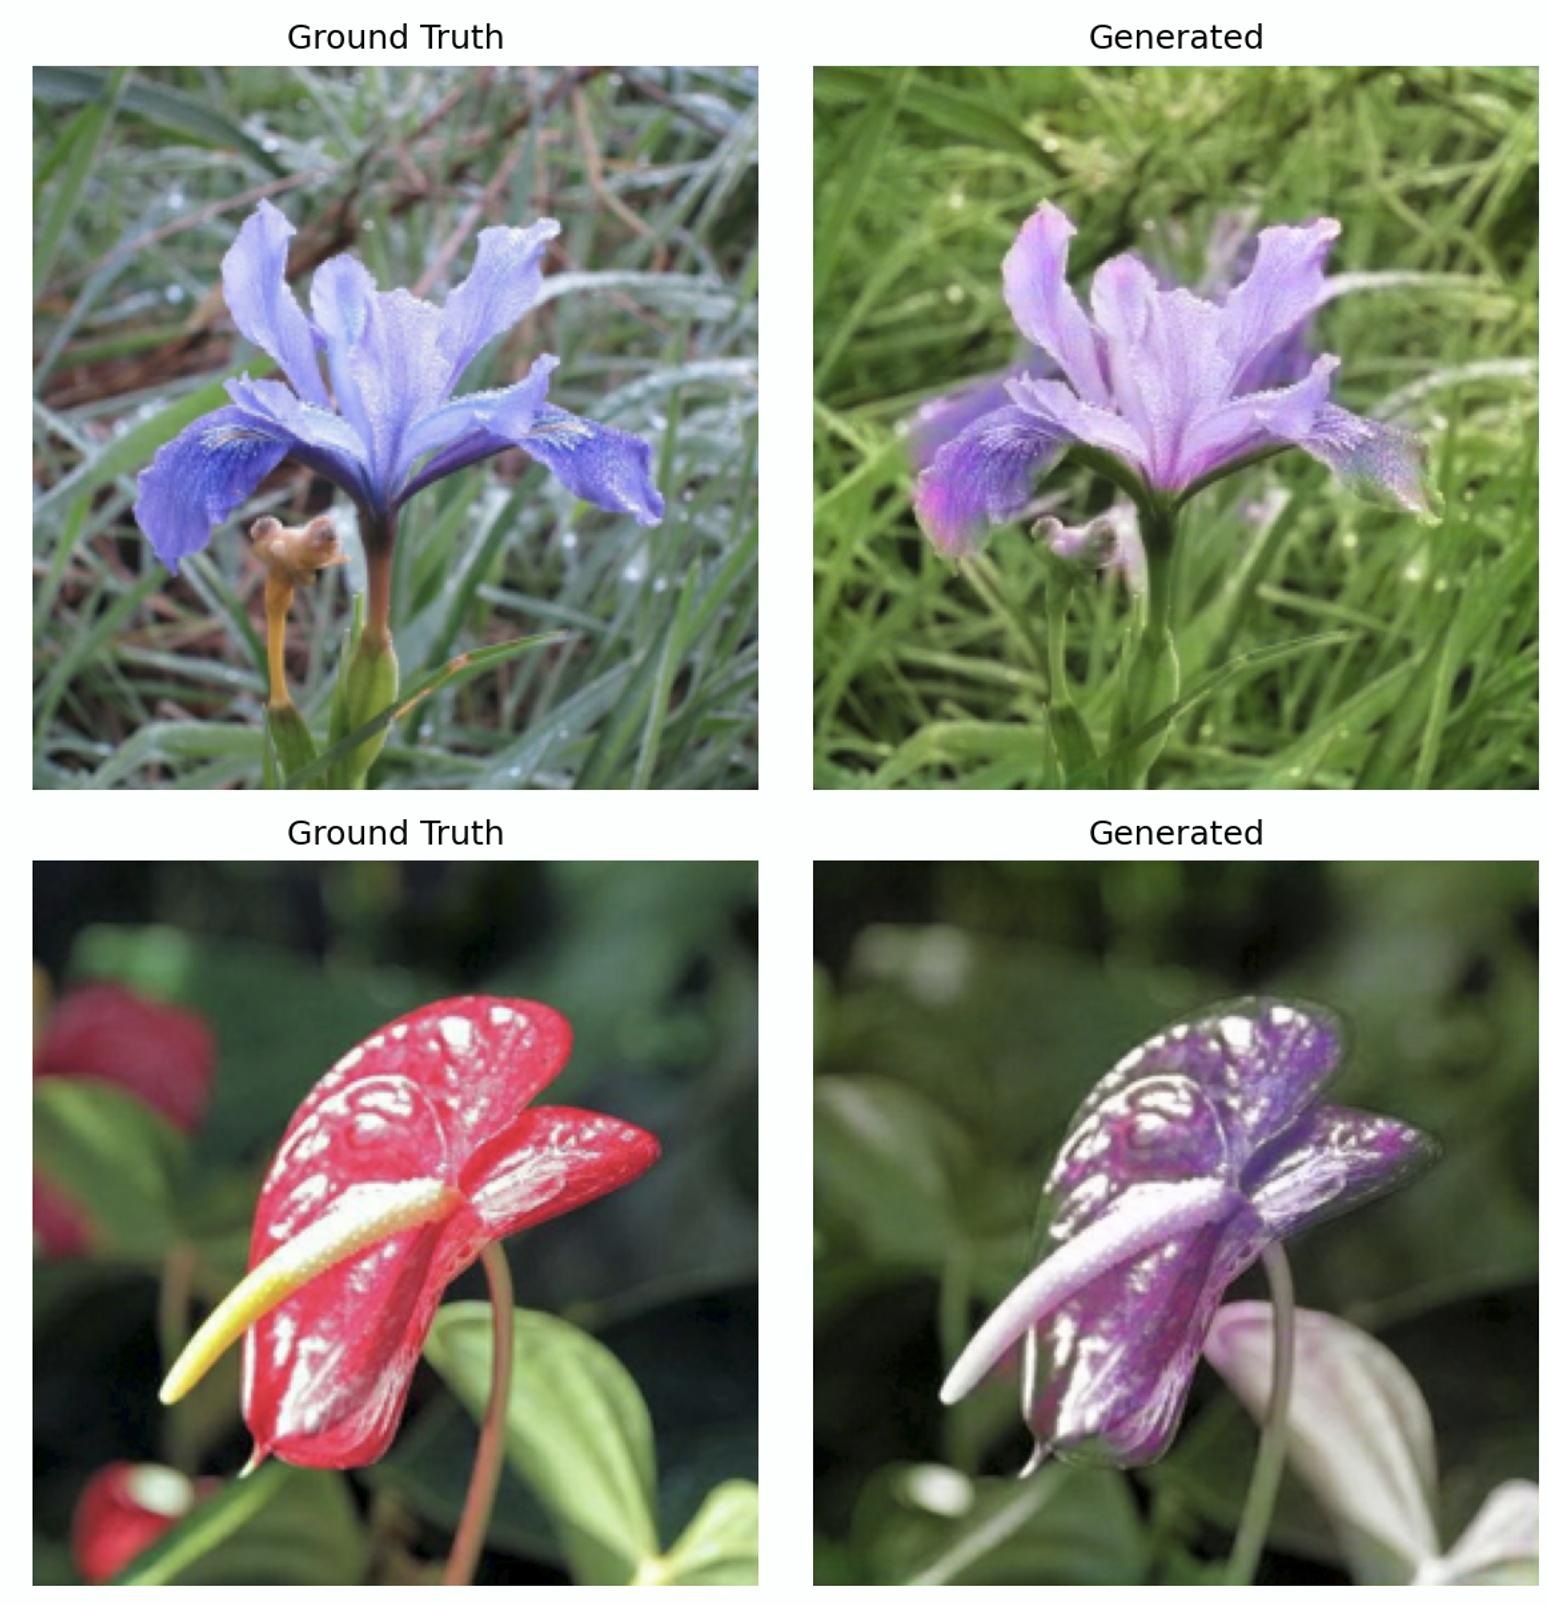
\includegraphics[width=0.9\textwidth, height=0.7\textheight, keepaspectratio]{img/lambda_et_lr_validation_epoch030.png}
        \caption{Validation avec réglage combiné $\lambda$ et LR }
    \end{figure}
\end{frame}

\begin{frame}{Résultats : Pondération manuelle et extension des Epochs}
    \begin{figure}
        \centering
        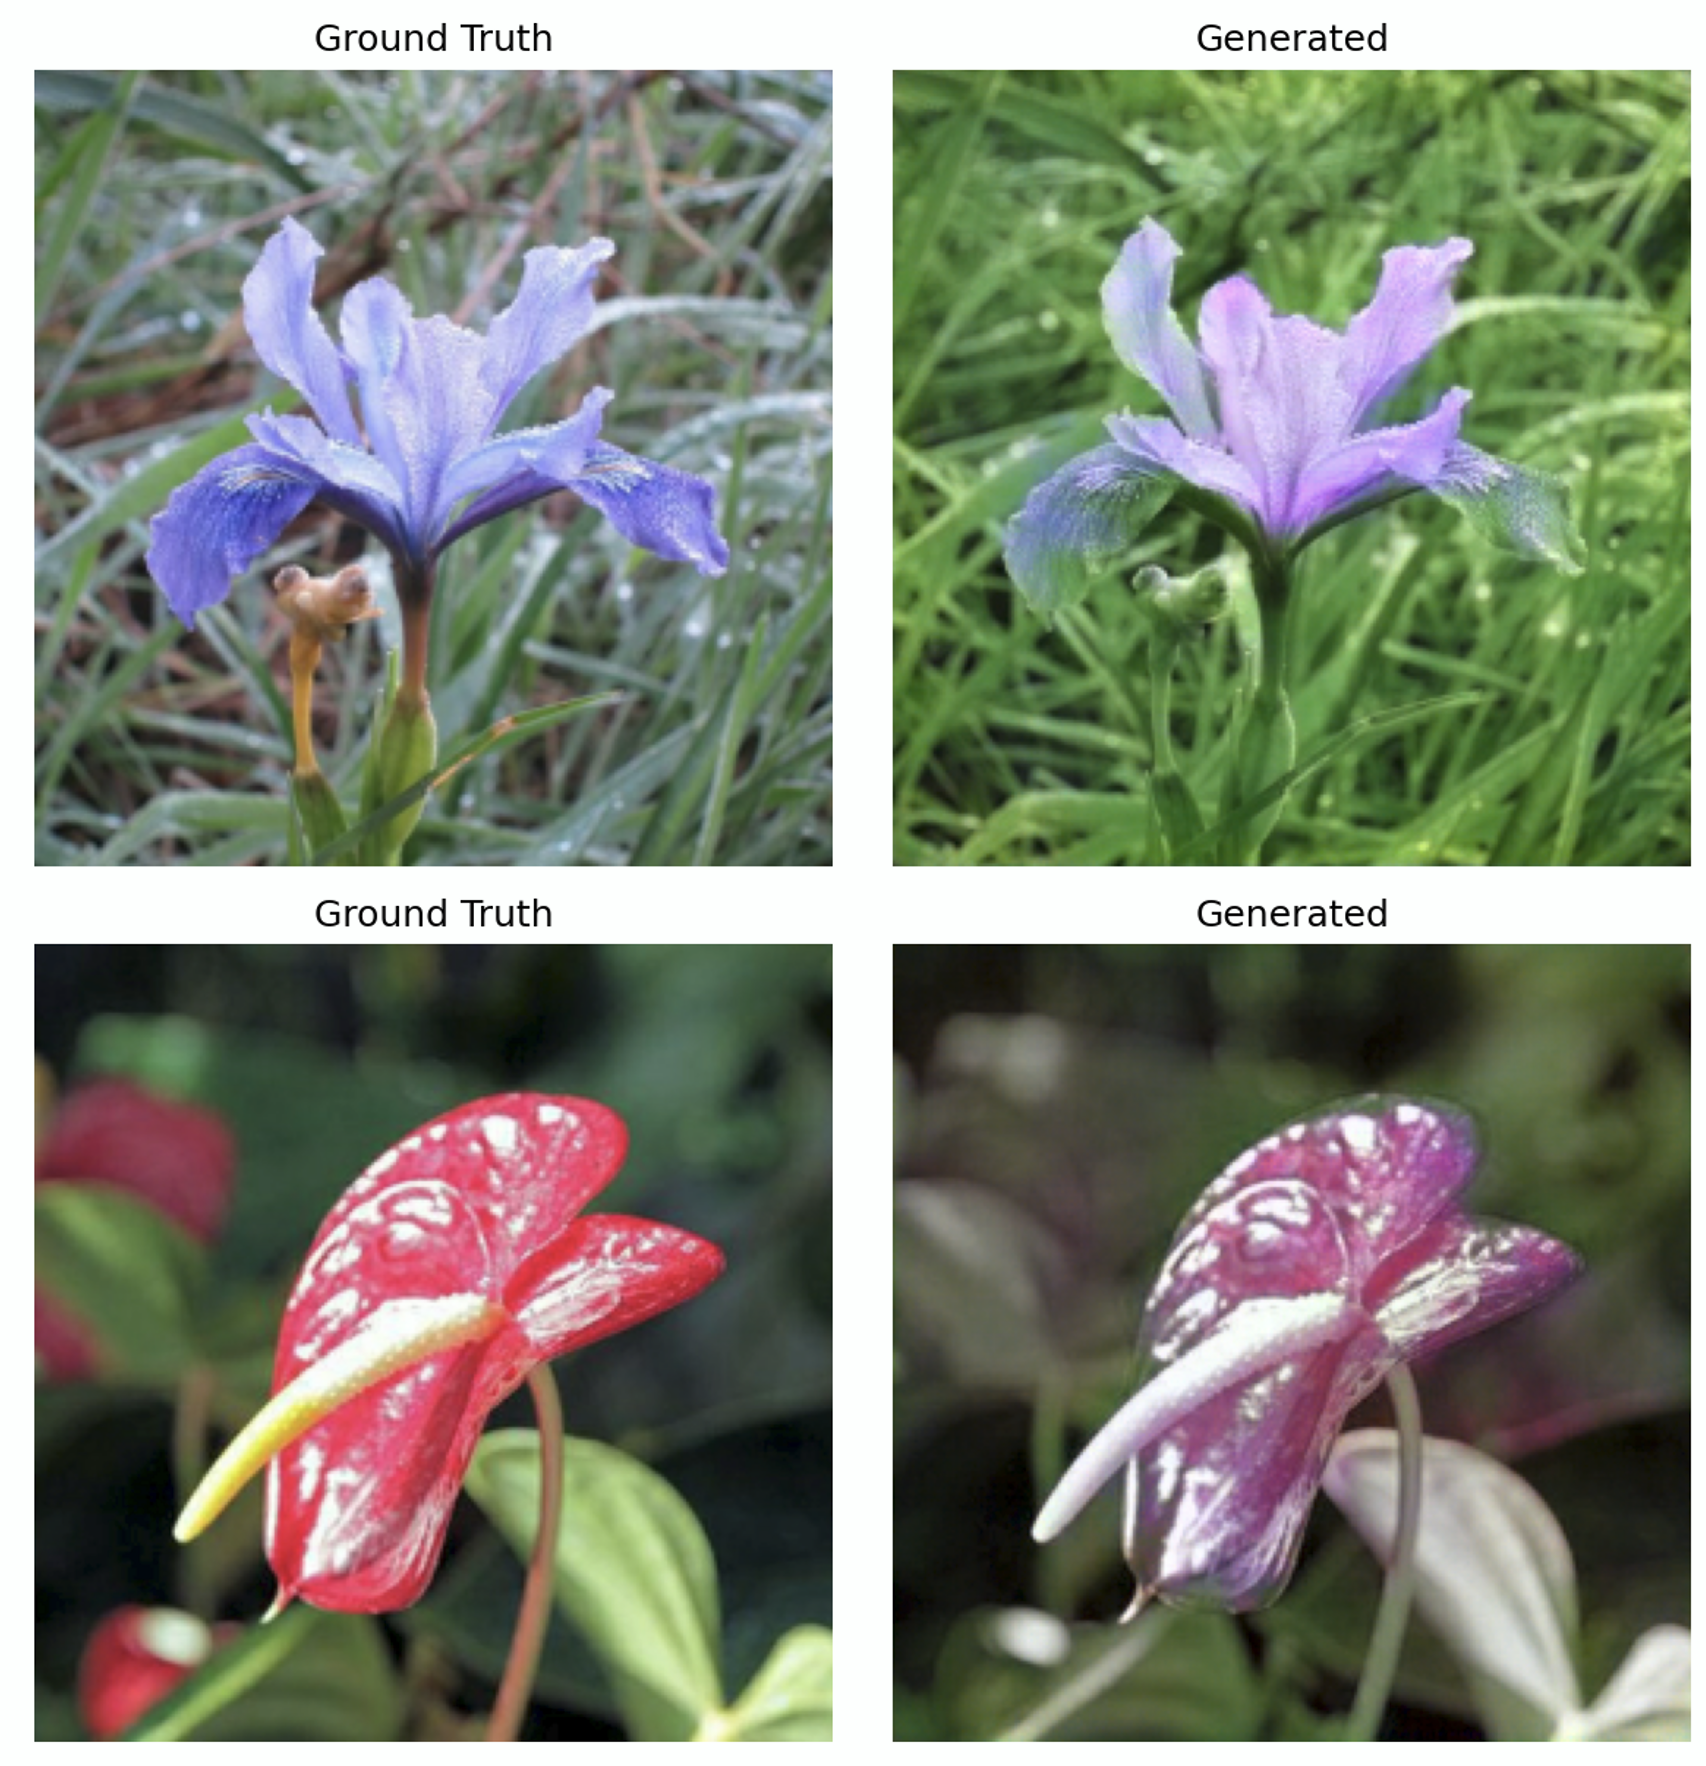
\includegraphics[width=0.9\textwidth, height=0.7\textheight, keepaspectratio]{img/ponderation_et_epoch_validation_epoch040.png}
        \caption{Validation avec pondération de la loss}
    \end{figure}
\end{frame}

\begin{frame}{Résultats : Intégration de la Perceptual Loss}
    \begin{figure}
        \centering
        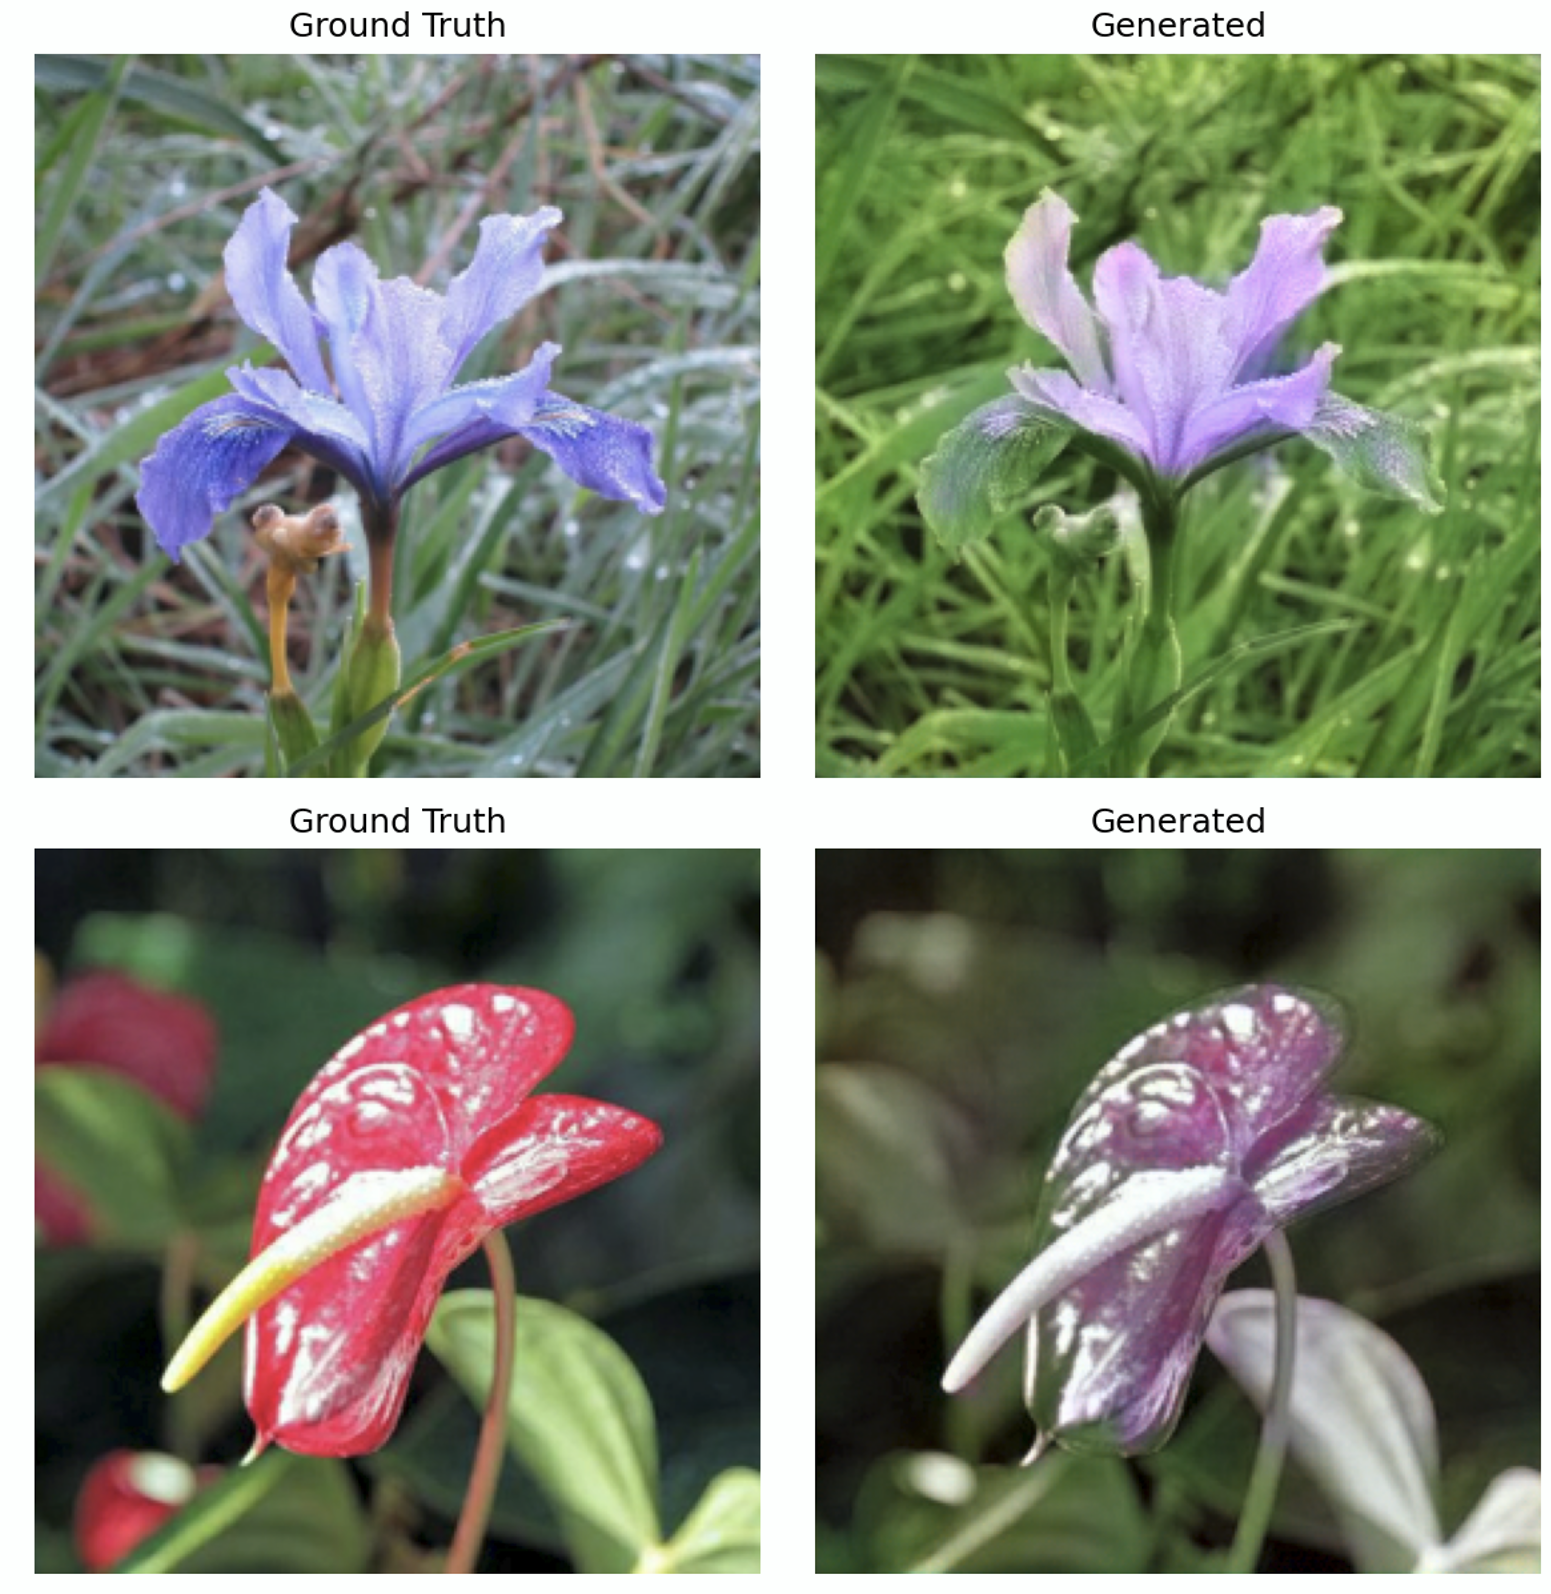
\includegraphics[width=0.9\textwidth, height=0.7\textheight, keepaspectratio]{img/perceptual_validation_epoch030.png}
        \caption{Validation avec Perceptual Loss}
    \end{figure}
\end{frame}

\begin{frame}{Tableau des métriques}

\begin{table}[h!]
    \centering
    \renewcommand{\arraystretch}{1.2}
    \setlength{\tabcolsep}{6pt} % Réduit l'espace entre les colonnes
    
    % Force le tableau à tenir sur la largeur de la diapositive
   \resizebox{\textwidth}{!}{
        \begin{tabular}{|l|c|l|l|c|c|c|}
            \hline
            \textbf{Nom de l'expérience} & \textbf{Époques} & \textbf{$\lambda$} & \textbf{LR} & \textbf{MAE} $\downarrow$ & \textbf{Acc.} ($\epsilon = 5\%$) $\uparrow$ & \textbf{Acc.} ($\epsilon = 10\%$) $\uparrow$ \\
            \hline
            Learning Rate & 20 & 100 & $lr_d: 2.0e-05, lr_g: 0.0002$ & 0.1094 & 13.85\% & 35.30\% \\
            \hline
            Lambda et LR & 40 & 10 & $lr_d: 2.0e-05, lr_g: 0.0002$ & 0.1403 & 12.58\% & 33.59\% \\
            \hline
            Pondération Manuelle & 40 & 100 & $lr_d: 2.0e-05, lr_g: 0.0002$ & 0.1240 & 14.72\% & 35.68\% \\
            \hline
            Perceptual Loss & 30 & $\lambda_{vgg}: 10, \lambda: 100$ & $lr_d: 2.0e-05, lr_g: 0.0002$ & 0.1299 & 13.76\% & 35.68\% \\
            \hline
        \end{tabular}
    }
    \caption{Comparaison des modèles selon les hyper-paramètres.}
\end{table}


\end{frame}

%Conclusion
%------------------------------------------------------------------------------------------------------------------------------------------------------------
\section{Conclusion}
\subsection{Ce qui a fonctionné / pas fonctionné}
%------------------------------------------------------------------------------------------------------------------------------------------------------------
\begin{frame}{Analyse des résultats : Restitution colorimétrique}
    \begin{itemize}
        \item \textbf{Performance globale :} Le modèle parvient à restituer les couleurs de manière approximative, validant la convergence de l'architecture.
        
        \item \textbf{Limitations constatées :}
        \begin{itemize}
            \item Les couleurs vives (rouge, violet) peinent à apparaître distinctement.
            \item Phénomène de lissage typique des fonctions de perte classiques qui privilégient les valeurs moyennes.
        \end{itemize}
        
        \item \textbf{Biais de données :}
        \begin{itemize}
            \item Forte prédominance du vert dans les résultats.
            \item Cause identifiée : Spécificité du dataset (fleurs) où la végétation occupe la majorité de l'espace pixel.
        \end{itemize}
    \end{itemize}
    
    \begin{alertblock}{Observation clé}
        Le modèle a tendance à se spécialiser sur la couleur la plus fréquente statistiquement pour minimiser la loss, au détriment des teintes minoritaires.
    \end{alertblock}

\end{frame}

\subsection{Amélioration possible}
%------------------------------------------------------------------------------------------------------------------------------------------------------------
\begin{frame}{Améliorations possibles}
    \begin{itemize}
        \item \textbf{Équilibrage du Dataset (Data Augmentation) :}
        \begin{itemize}
            \item Introduire des transformations de couleur pour réduire le biais lié au vert.
            \item Intégrer des images plus diversifiées pour équilibrer la distribution statistique des classes chromatiques.
        \end{itemize}

        \item \textbf{Optimisation de la fonction de perte :}
        \begin{itemize}
            \item Ajuster les poids de la Perceptual Loss pour forcer le modèle à reconstruire les détails fins et les contrastes de couleurs.
        \end{itemize}
        \item \textbf{Pré-entraînement :}
        \begin{itemize}
            \item Utiliser un dataset plus diversifié et plus complet, puis spécialiser le modèle sur les fleurs.
        \end{itemize}
    \end{itemize}
\end{frame}

\subsection{Impact sociétal}
%------------------------------------------------------------------------------------------------------------------------------------------------------------
\begin{frame}{Impact sociétal et enjeux de la colorisation}
    \small % Réduit légèrement la taille du texte pour tout faire tenir
    \begin{itemize}
        \item \textbf{Patrimoine :} Préserver le patrimoine en restaurant des images d'époque.
        
        \item \textbf{Applications techniques :} Aide à l'analyse d'imagerie médicale et satellite
    \end{itemize}

    \vspace{0.2cm} % Petit espace pour respirer

    \begin{block}{Optimisation du stockage et compression}
        \footnotesize % Le bloc peut être écrit plus petit car c'est une conclusion technique
        L'approche permet une compression drastique : en ne stockant que le canal de luminance $L$ (gris), l'IA reconstruit l'information chromatique ($a, b$) à la volée, réduisant théoriquement le poids des fichiers de 2/3.
    \end{block}
\end{frame}

%Annexes
%------------------------------------------------------------------------------------------------------------------------------------------------------------
\section{Annexes}


\subsection{Analyse du problème}

%------------------------------------------------------------------------------------------------------------------------------------------------------------

\begin{frame}{Analyse de nos entrées}

\begin{columns}[c] % [c] pour l'alignement vertical centré
        
        % Colonne de gauche : Image Noir et Blanc
        \begin{column}{0.37\textwidth}
            \begin{figure}
                \centering
                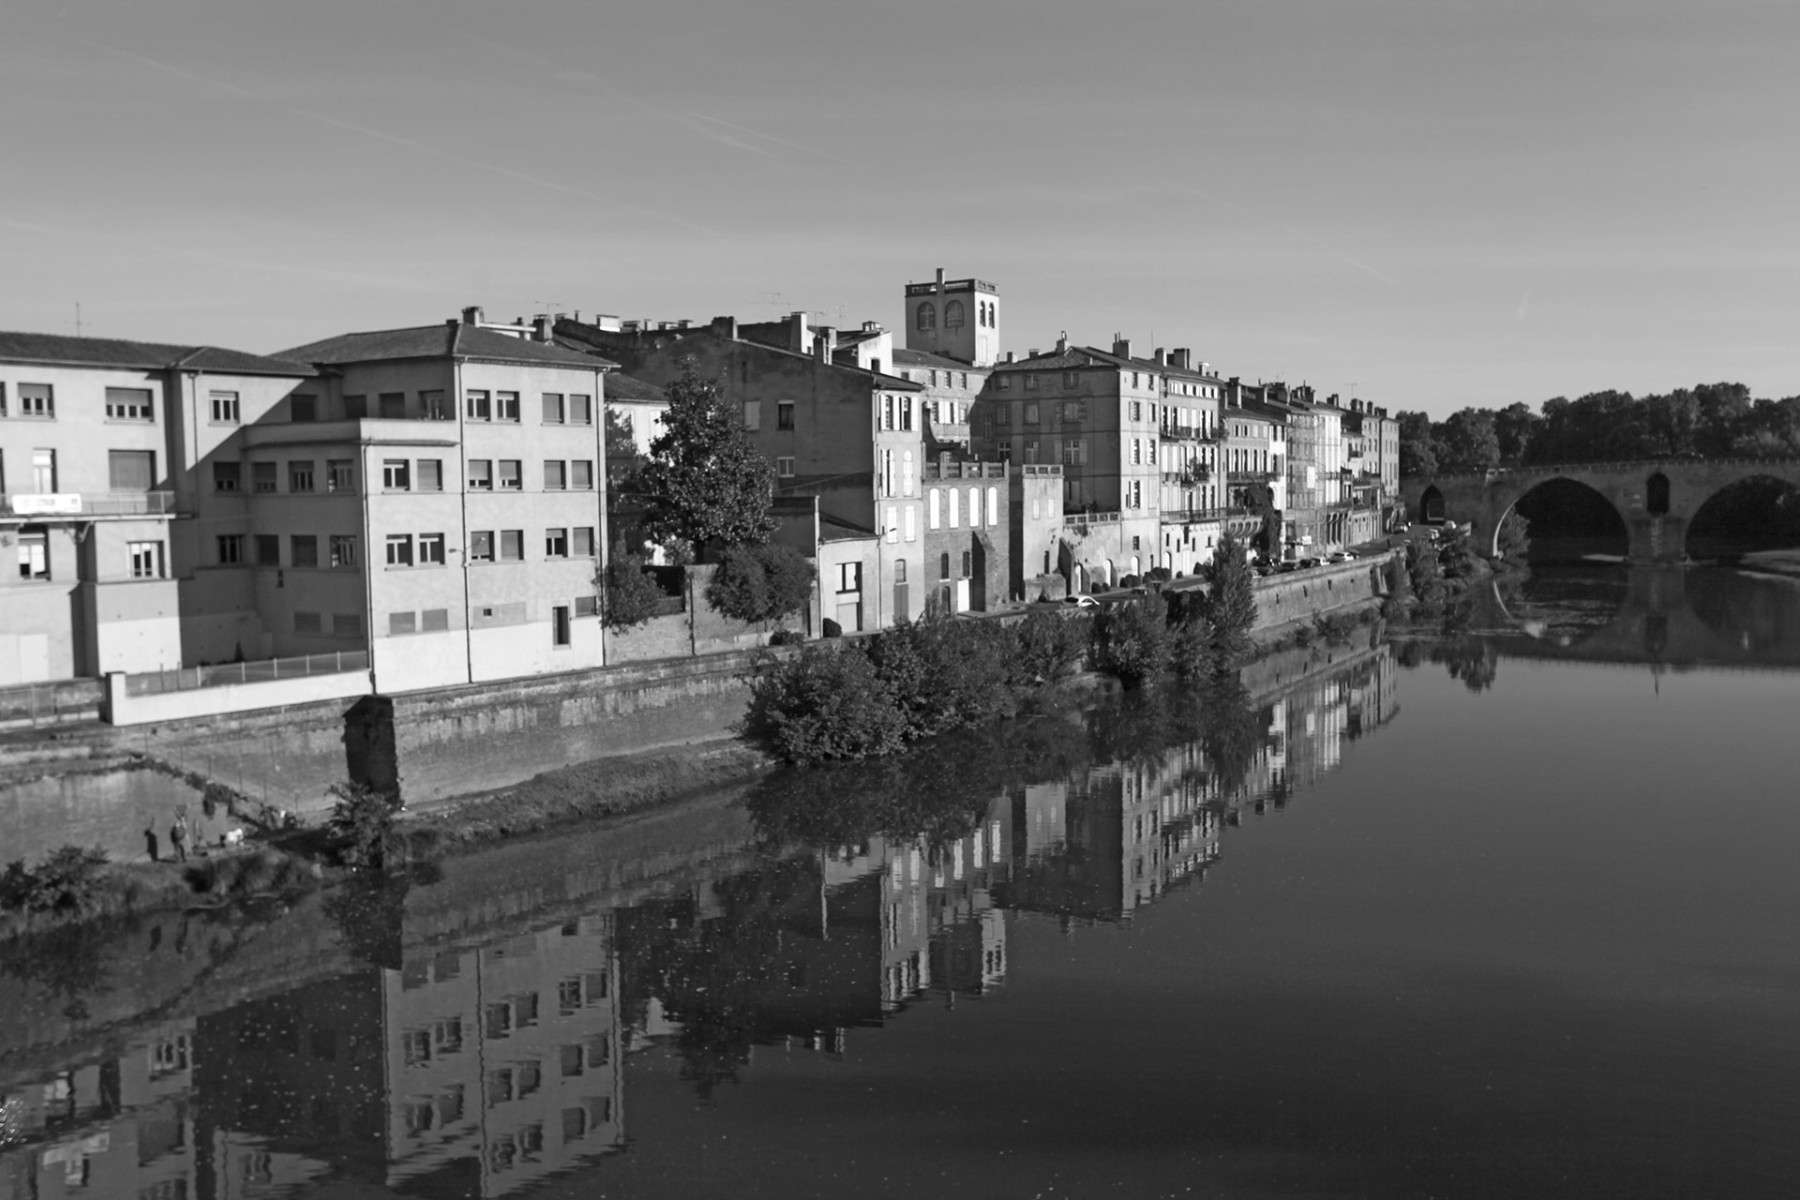
\includegraphics[width=\textwidth]{img/image_exemple_NB.jpg}
                \caption{Image d'entrée (N\&B)}
            \end{figure}
        \end{column}

        % Colonne de droite : Image Colorisée
        \begin{column}{0.50\textwidth}
        \begin{table}[h]
        \centering
        \begin{tabular}{|l|l|}
            \hline
            \textbf{Catégorie} & \textbf{Nos entrées} \\ \hline
            \textbf{Nature} & Pixels  \\ \hline
            \textbf{Forme} & Images de 256*256*1  \\ \hline
            \textbf{Dimensions} & Fixes \\ \hline
        \end{tabular}
        \caption{Récapitulatif de nos entrées}
        \end{table}
        \end{column}

\end{columns}
\end{frame}

%------------------------------------------------------------------------------------------------------------------------------------------------------------

\begin{frame}{Analyse de nos sorties}
\begin{columns}[c] % [c] pour l'alignement vertical centré
        
        % Colonne de gauche : Image Noir et Blanc
        \begin{column}{0.37\textwidth}
            \begin{figure}
                \centering
                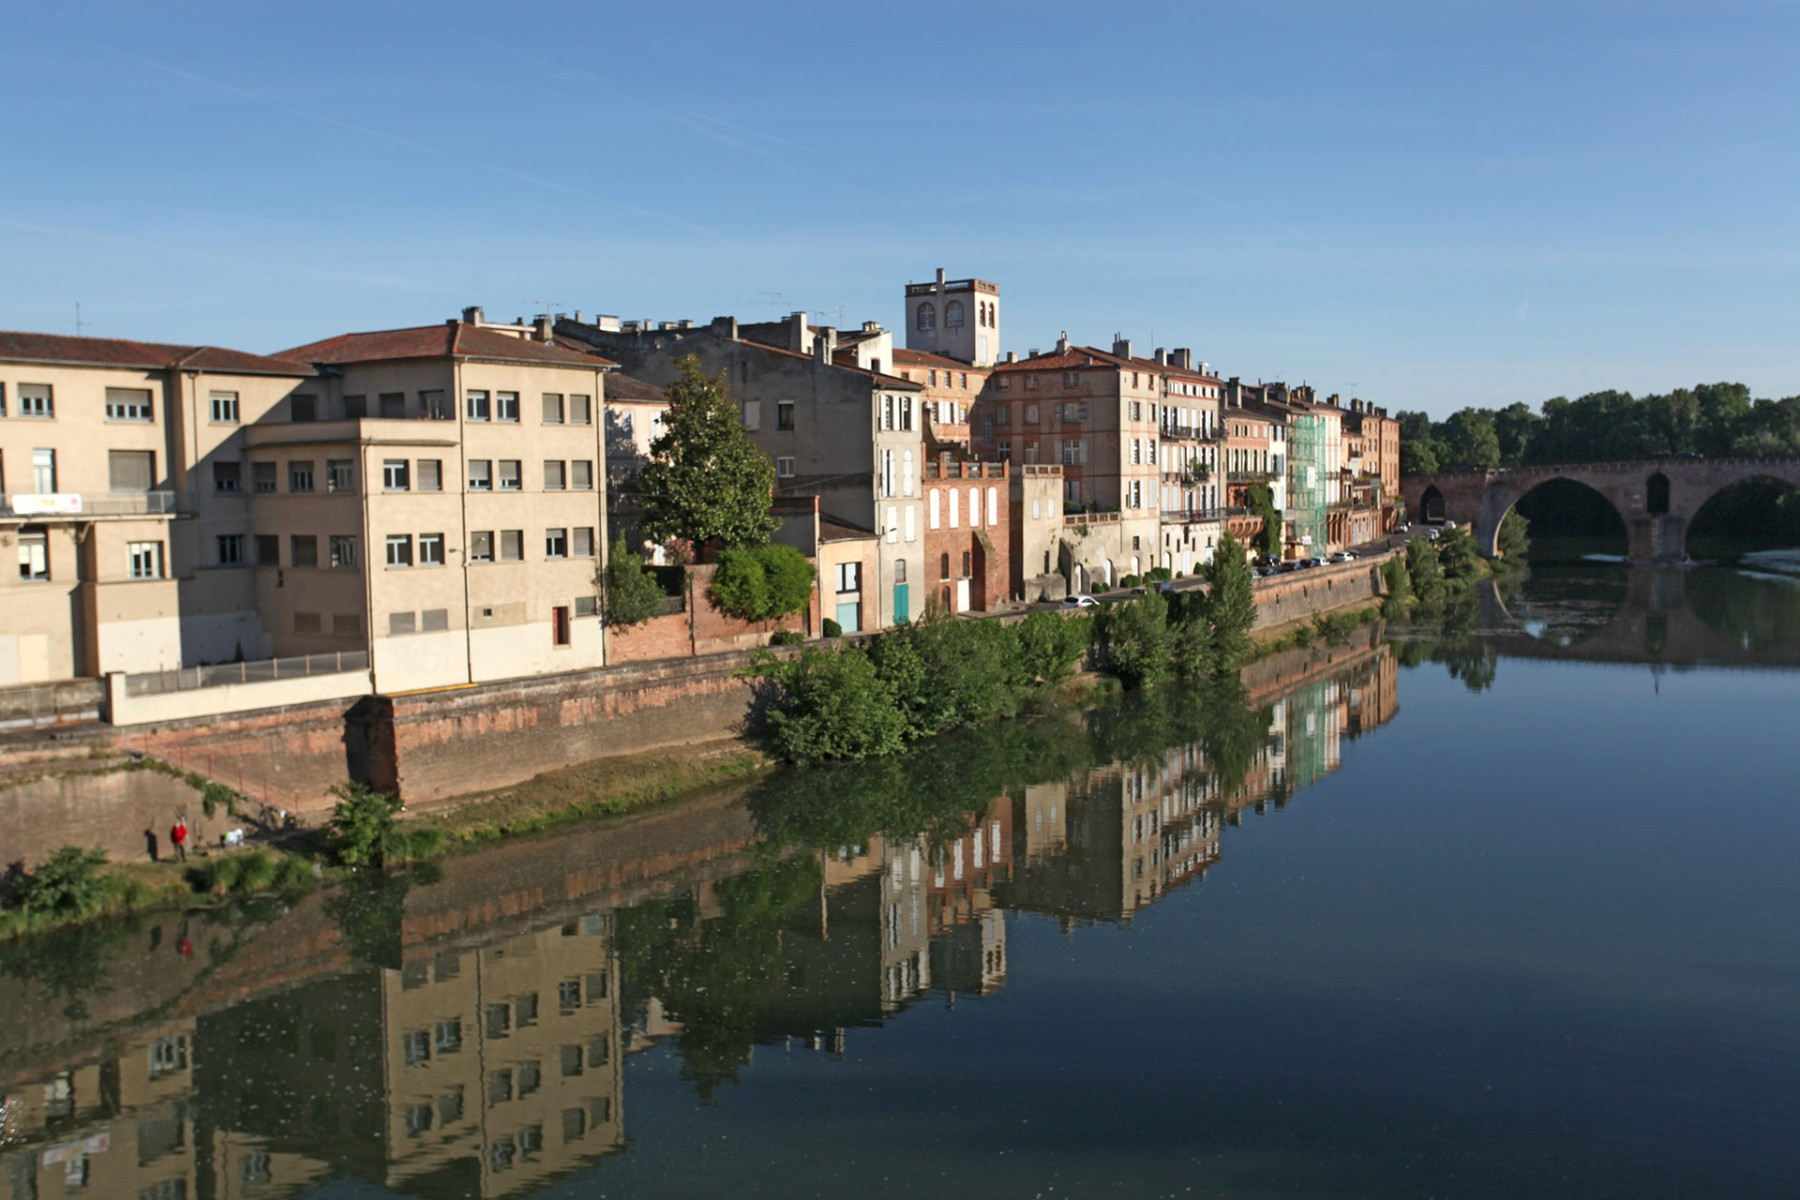
\includegraphics[width=\textwidth]{img/image_exemple_couleur.jpg}
                \caption{Image de sortie (Couleur)}
            \end{figure}
        \end{column}

        % Colonne de droite : Image Colorisée
        \begin{column}{0.50\textwidth}
        \begin{table}[h]
        \centering
        \begin{tabular}{|l|l|}
            \hline
            \textbf{Catégorie} & \textbf{Nos sorties} \\ \hline
            \textbf{Nature} & Pixels  \\ \hline
            \textbf{Forme} & Images de 256*256*3  \\ \hline
            \textbf{Dimensions} & Fixes \\ \hline
        \end{tabular}
        \caption{Récapitulatif de nos sorties}
        \end{table}
        \end{column}

\end{columns}

\end{frame}

\subsection{Formulation mathématiques}
%------------------------------------------------------------------------------------------------------------------------------------------------------------

\begin{frame}{Formalisation du problème de ML}
    Soit une image d'entrée $X \in \mathbb{R}^{H \times W \times 1}$ représentant le canal $L$. 
    Le but est d'apprendre une fonction $f$ pour prédire les canaux de chrominance $Y$ :
    $$\hat{Y} = f(X) \quad \text{où} \quad \hat{Y} \in \mathbb{R}^{H \times W \times 2}$$
    
        \vfill 
    
    L'image finale colorisée est la concaténation de l'entrée et du résultat : 
$$I_{\text{final}} = [X, \hat{Y}]$$
    
\end{frame}

\subsection{Approches déterministes}


%------------------------------------------------------------------------------------------------------------------------------------------------------------

\begin{frame}{Algorithme de matching}

Proposé en 2002 par \textbf{Welsh et al.} \footcite{welsh2002} :

\vfill

\begin{center}
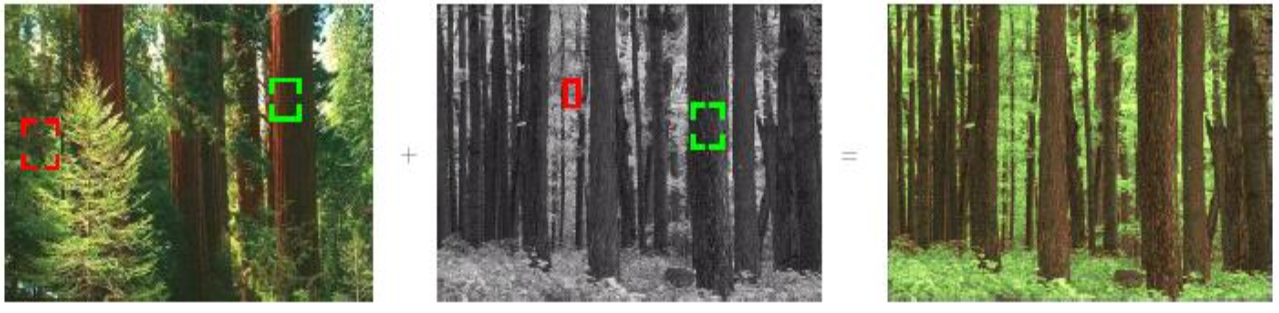
\includegraphics[width=0.8\linewidth]{texture.PNG}
\end{center}

\vfill

\begin{alertblock}{Limites du modèle}
\begin{itemize}
\item \textbf{Problème déterministe :} Pour un réglage donné, le résultat est unique et figé.
\item \textbf{Intervention humaine}
\item \textbf{Incertitude}
\end{itemize}
\end{alertblock}

\end{frame}

%------------------------------------------------------------------------------------------------------------------------------------------------------------

\begin{frame}{Algorithme de d'optimisation}

    Proposé en 2002 par \cite{levin2004}
    
\end{frame}

%------------------------------------------------------------------------------------------------------------------------------------------------------------


\end{document}

